% latex article template

% cheat sheet(eng): http://www.pvv.ntnu.no/~walle/latex/dokumentasjon/latexsheet.pdf
% cheat sheet2(eng): http://www.pvv.ntnu.no/~walle/latex/dokumentasjon/LaTeX-cheat-sheet.pdf
% reference manual(eng): http://ctan.uib.no/info/latex2e-help-texinfo/latex2e.html

\documentclass[12pt, a4paper]{article}
\title{TDT4300 - Assignment 1}

\PassOptionsToPackage{hyphens}{url}
\usepackage[pdfborder=0 0 0]{hyperref}
\usepackage[utf8]{inputenc}
\usepackage[english]{babel}
\usepackage{graphicx}

% hides the section numbering. 
\setcounter{secnumdepth}{-1}

% Graphics/image lications and extensions. 
\DeclareGraphicsExtensions{.pdf, .png, .jpg, .jpeg}
\graphicspath{{./images/}}

% Author
\author{
        Magnus L Kirø \\
}
\date{\today}

\begin{document}
\maketitle
\pagenumbering{arabic}


\section{ex1}
a) 
OLTP are a series of short online transactions. The emphasis is mainly on fast query processing. 
OLAP has a low volume of transactions, but the queries are complex, which means that fewer queries are required. 

b) 
A data cube is an array that has three or more dimensions. 
A cuboid is a cube formed set of data. Might refer to a dataset og a result from a query. 

c) 
Explain the data cube operations slice, dice, rollup and drill-down.

Slice: take of a tiny part of the cube. Often removing a side of the cube for analysis. 
Dice: split the datacube into multiple smaller datacubes. 
rollup: put together slices of data to create a cube. 
drill-down: taking out a portion of the cubes middle. Often just a single value, og a dice.

\section{ex2}

Star diagram: \ref{fig1}
% imgae example. 
\begin{figure}[htb]
    \centering
    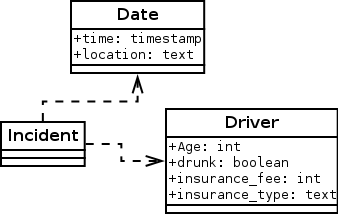
\includegraphics[width=\textwidth]{star1}
    \caption{Star - diagram - ex2}
    \label{fig1}
\end{figure}

snowflake: \ref{fig2}
% imgae example. 
\begin{figure}[htb]
    \centering
    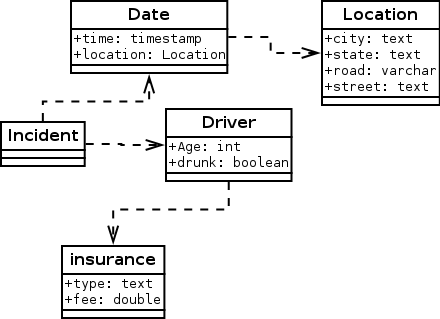
\includegraphics[width=\textwidth]{snowflake}
    \caption{Snowflake - diagram - ex2}
    \label{fig2}
\end{figure}

concept 1: \ref{con1}
% imgae example. 
\begin{figure}[htb]
    \centering
    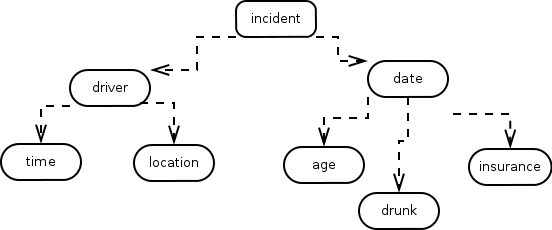
\includegraphics[width=\textwidth]{concept1}
    \caption{Concept hierarchy - ex2}
    \label{con1}
\end{figure}

concept 2: \ref{con2}
% imgae example. 
\begin{figure}[htb]
    \centering
    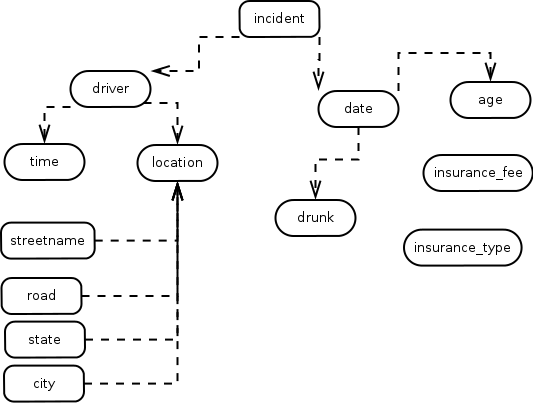
\includegraphics[width=\textwidth]{concept2}
    \caption{Concept hierarchy - ex2}
    \label{con2}
\end{figure}




\section{ex3}
a)
Stardiagram: \ref{fig5}
% imgae example. 
\begin{figure}[htb]
	\centering
	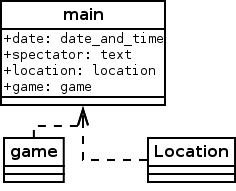
\includegraphics[width=\textwidth]{game}
	\caption{Star - diagram - ex3}
	\label{fig5}
\end{figure}

b) 
slice the cube to get all participants that are students.
dice the cube to get alle the participants that are students and was at the specific arena.
slice the remaining cube to remove the students that wasn't visiting in the wanted time period. 
drill to get the fee from all of the remaining participants. 
sum the remaining fields.

c)
Bitmaps in this setting might be a bit much. 
The datastructure is small and the data is uneven. 
Spectator does not have as much information as location and game. 
Bitmaps are good with square regular data. 


\end{document}
